\documentclass[A4]{article}

\usepackage[14pt]{extsizes}
\usepackage{graphicx}
\graphicspath{ {./images/} }
\usepackage{amsfonts}
\usepackage[T2A]{fontenc}
\usepackage[utf8]{inputenc}
\usepackage[russian]{babel}
\usepackage{amsmath}%
\usepackage{MnSymbol}%
\usepackage{wasysym}%
\usepackage{arcs}
\usepackage{indentfirst}
\usepackage[left = 1.5cm, right = 1.5cm, top = 1cm]{geometry}

\usepackage{amsmath}

\title{\textbf{Статистики Ферми-Дирака и Бозе-Эйнштейна}\\
       Вопрос по выбору для экзамена по курсу\\
       "Общая физика: термодинамика и молекулярная физика"}
\author{Григорьев Даниил, Б01-407}
\date{}

\begin{document}

\maketitle

\newpage
\section{Аннотация}

    Распределение Больцмана выводится в предположении, что любые две частицы принципиально
    различимы, даже если они тождественны. В рамках квантовой механики такое утверждение оказывается
    неверным, и нужно искать новый вид распределения. Этому и посвящена данная работа.

\section{Введение}

    Согласно квантовой механике, все частицы можно разделить на две группы по величине спина
    \footnote{Спин - собственный момент импульса частицы, имеющий квантовую природу. Спин измеряется в
    величинах $n\cdot\hbar$, где $n$ - целое или полуцелое число, называемое спиновым квантовым числом}.
    Частицы с целым спином называются \textbf{бозонами} и подчиняются статистике Бозе-Эйнштейна.
    Частицы с полуцелым спином называются \textbf{фермионами} и подчиняются статистике Ферми-Дирака.

    \begin{center}
        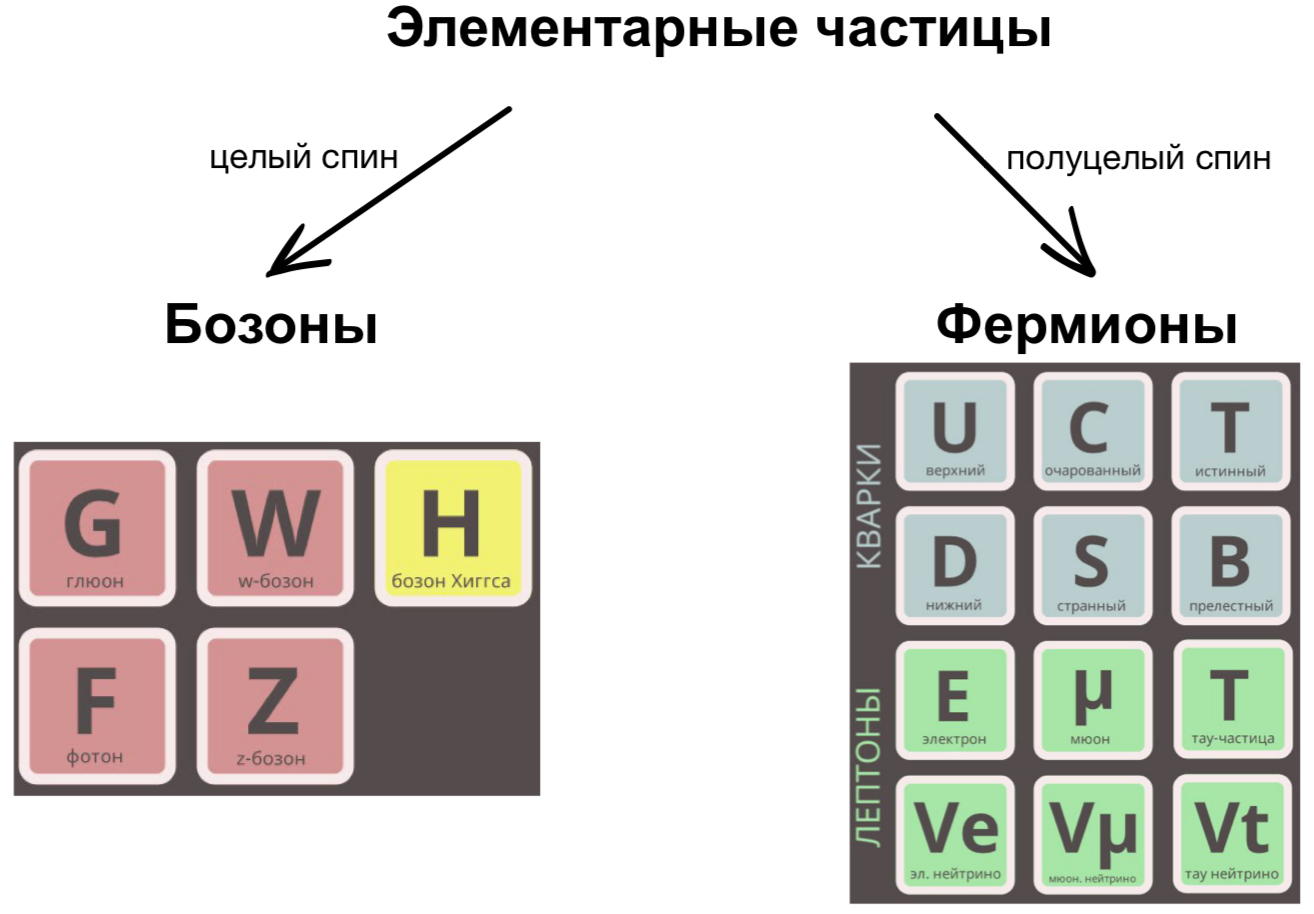
\includegraphics[width=13cm]{elementary.png}
    \end{center}

    В обеих статистиках допустимые микросостояния системы принимаются равновероятными и тождественные
    частицы считаются неразличимыми. Различие между статистиками следующее. В статистике Ферми-Дирака
    принимается, что в каждом квантовом состоянии может находиться не более одной частицы. Статистика
    Бозе-Эйнштейна таких ограничений не накладывает. Причины такого различного поведения бозонов и
    фермионов объясняются в квантовой механике и автору неизвестны.

\section{Необходимые сведения из комбинаторики}

    Найдём число способов распределить N тождественных частиц по Z квантовым состояниям.

    В одном квантовом состоянии может находиться не более одного фермиона, поэтому задача сводится к поиску
    числа способов разместить N объектов по Z ячейкам без повторений и без учёта порядка. Это число равно:
    \begin{equation*}
        C_Z^N = \frac{Z!}{N!(Z - N)!}
    \end{equation*}

    Поскольку в одном квантовом состоянии может быть более одного бозона, то для этих частиц задача сводится
    к поиску числа способов разместить N объектов по Z ячейкам с повторениями и без учёта порядка. Это число
    равно:
    \begin{equation*}
        C_{Z + N - 1}^N = \frac{(Z + N - 1)!}{N!(Z - 1)!}
    \end{equation*}

\section{Распределения Ферми-Дирака и Бозе-Эйнштейна}

    В качестве модели будем рассматривать "идеальный газ"\ из фермионов (ферми-газ) или бозонов (бозе-газ),
    помещённый в сосуд постоянного объёма с твёрдыми и непроницаемыми адиабатическими стенками.

    Макросостояние газа будем характеризовать следующим образом. Разделим все квантовые состояния на
    "энергетические слои"\ так, чтобы энергии квантовых состояний в $i$-м слое принадлежали промежутку
    $(\varepsilon_i,\ \varepsilon_i + \delta\varepsilon_i)$, где $\delta\varepsilon_i \ll \varepsilon_i$.
    Также потребуем, чтобы число квантовых состояний $Z_i$ в $i$-м слое было велико ($Z_i \gg 1$).
    Макросостояние будет характеризоваться числом $N_i$ частиц в каждом слое. Не теряя общности, будем
    считать, что никакое квантовое состояние не является вырожденным\footnote{Квантовое состояние
    называется вырожденным, если существует несколько состояний частицы с тем же значением энергии,
    отличающихся другими физическими величинами}. Если это не так, то достаточно разделить каждый
    кратный уровень на соответствующие простые подуровни, чтобы свести реальные случай к рассматриваемому.

    Число способов распределить $N_i$ частиц по $Z_i$ квантовым состояниям $i$-го слоя равно:
    \begin{equation*}
        G_i^{(\text{ф})} = \frac{Z_i!}{N_i!(Z_i - N_i)!};\ \ \ G_i^{(\text{б})} = \frac{(Z_i + N_i - 1)!}{N_i!(Z_i - 1)!}
    \end{equation*}

    Пусть число частиц фиксировано для каждого энергетического слоя, тогда при любых их распределениях
    по квантовым состояниям макросостояние будет оставаться прежним. Отсюда получаем, что для
    фиксированных $N_i$ статистический вес макросостояния определяется выражениями:
    \begin{equation}\label{statistical weight}
        G^{(\text{ф})} = \prod\limits_{i}\frac{Z_i!}{N_i!(Z_i - N_i)!};\ \ \
        G^{(\text{б})} = \prod\limits_{i}\frac{(Z_i + N_i - 1)!}{N_i!(Z_i - 1)!}
    \end{equation}

    По постановке задачи объём и внутренняя энергия как ферми-газа, так и бозе-газа являются постоянными
    величинами. Поэтому имеем ещё два уравнения:
    \begin{equation}\label{const_n}
        \sum\limits_{i} N_i = N = const
    \end{equation}
    \begin{equation}\label{const_e}
        \sum\limits_{i} N_i\varepsilon_i = E = const
    \end{equation}

    Найдём такое распределение частиц по квантовым состояниям, которому соответствует максимум
    выражения \eqref{statistical weight} при условиях \eqref{const_n} и \eqref{const_e}. В таком
    случае энтропия системы будет также максимальной, а значит, система будет пребывать в состоянии
    устойчивого термодинамического равновесия. По формуле Больцмана:
    \begin{equation}\label{FD_1}
        \begin{split}
            S^{(\text{ф})} = k\ln{G^{(\text{ф})}} + C =
            k\ln{\left(\prod\limits_{i}\frac{Z_i!}{N_i!(Z_i - N_i)!}\right)} + C =
            k\sum\limits_{i} \ln{\frac{Z_i!}{N_i!(Z_i - N_i)!}} + C = \\\\
            = k\sum\limits_{i}(\ln{Z_i!} - \ln{N_i!} - \ln{(Z_i - N_i)!}) + C =
            -k\sum\limits_{i}(\ln{N_i!} + \ln{(Z_i - N_i)!}) + C.
        \end{split}
    \end{equation}

    Теперь предположим, что также все $N_i \gg 1$. Заметим, что это условие не может быть выполнено
    для всех $N_i$. Несмотря на то что $N$ велико, оно конечно, следовательно некоторые $N_i$
    неизбежно окажутся равными 0 при достаточно больших $i$. Тем не менее число таких молекул
    много меньше $N$, и их присутствие пренебрежимо мало сказывается на статистическом поведении
    газа. Таким образом, мы обосновали возможность применения формулы Стирлинга (далее $N$ - это
    $N_i$ или $Z_i$):
    \begin{equation*}
        N! \approx \sqrt{2\pi N}\left(\frac{N}{e}\right)^N
    \end{equation*}
    Для логарифма факториала имеем:
    \begin{equation*}
        \ln{N!} \approx \frac{1}{2}\ln{2\pi} + \left(N + \frac{1}{2}\right)\ln{N} - N
    \end{equation*}
    Первое слагаемое в правой части одинаково для всех $N_i$ и $Z_i$. Также в силу того, что
    $N_i \gg 1$ и $Z_i \gg 1$, можно приближённо написать $N + \frac{1}{2} \approx N$. Окончательно
    имеем:
    \begin{equation}\label{approximation}
        \ln{N!} \approx C + N\ln{N} - N
    \end{equation}
    Подставим \eqref{approximation} в \eqref{FD_1}:
    \begin{equation}\label{FD_2}
    \begin{split}
        S^{(\text{ф})} = -k\sum\limits_{i}N_i\ln{N_i} + k\sum\limits_{i}N_i -
        k\sum\limits_{i}(Z_i - N_i)\ln{(Z_i - N_i)} + k\sum\limits_{i}(Z_i - N_i) + C = \\\\
        = -k\sum\limits_{i}N_i\ln{N_i} - k\sum\limits_{i}(Z_i - N_i)\ln{(Z_i - N_i)} +
        k\sum\limits_{i}Z_i + C = \\\\ = -k\sum\limits_{i}[N_i\ln{N_i} + (Z_i - N_i)\ln{(Z_i - N_i)}] + C.
    \end{split}
    \end{equation}
    Аналогично можно получить выражение для энтропии бозе-газа:
    \begin{equation*}
        S^{(\text{б})} = -k\sum\limits_{i}[(Z_i + N_i - 1)\ln{(Z_i + N_i - 1)} - N_i\ln{N_i}] + C
    \end{equation*}
    Так как $N_i \gg 1$, то в последнем выражении единицей можно пренебречь и оно примет вид:
    \begin{equation}\label{BE}
        S^{(\text{б})} = -k\sum\limits_{i}[(Z_i + N_i)\ln{(Z_i + N_i)} - N_i\ln{N_i}] + C
    \end{equation}
    Введём обозначения:
    \begin{equation*}
        f(N_1, ..., N_n) = \sum\limits_{i}^{n} [N_i\ln{N_i} + (Z_i - N_i)\ln{(Z_i - N_i)}]
    \end{equation*}
    \begin{equation*}
        \varphi_1(N_1, ..., N_n) = - N + \sum\limits_{i} N_i \equiv 0
    \end{equation*}
    \begin{equation*}
        \varphi_2(N_1, ..., N_n) = - E + \sum\limits_{i} \varepsilon_i N_i \equiv 0
    \end{equation*}
    Запишем функцию Лагранжа:
    \begin{equation*}
        L(N_1, ..., N_n) = f(N_1, ..., N_n) + \lambda_1\varphi_1(N_1, ..., N_n) +
        \lambda_2\varphi_2(N_1, ..., N_n)
    \end{equation*}
    Найдём частные производные функции Лагранжа по всем переменным:
    \begin{equation*}
        \frac{\partial L}{\partial N_i} = \frac{\partial f}{\partial N_i} +
        \lambda_1\frac{\partial \varphi_1}{\partial N_i} +
        \lambda_2\frac{\partial \varphi_2}{\partial N_i} =
        \ln{\frac{N_i}{Z_i - N_i}} + \lambda_1 + \varepsilon_i\lambda_2
    \end{equation*}
    Согласно необходимому условию условного локального экстремума, найдутся такие $\lambda_1$ и
    $\lambda_2$, что точка условного локального экстремума функции $f$ является стационарной точкой
    функции $L$. Значит, в этой точке все частные производные функции $L$ равны нулю. Таким образом,
    имеем условие, что для всех $i$ выполняется:
    \begin{equation*}
        \ln{\frac{N_i}{Z_i - N_i}} + \lambda_1 + \varepsilon_i\lambda_2 = 0
    \end{equation*}
    Откуда получаем:
    \begin{equation*}
        \frac{\overline{N_i}}{Z_i - \overline{N_i}} = e^{-\lambda_1}e^{-\lambda_2\varepsilon_i}
    \end{equation*}
    Черта сверху показывает, что величина взята для наиболее вероятного состояния системы.
    Введём новую константу $A = e^{-\lambda_1}$, тогда последнее выражение примет вид:
    \begin{equation*}
        \frac{\overline{N_i}}{Z_i - \overline{N_i}} = Ae^{-\lambda_2\varepsilon_i}
    \end{equation*}
    Аналогично для статистики Бозе-Эйнштейна:
    \begin{equation*}
        \frac{\overline{N_i}}{Z_i + \overline{N_i}} = Ae^{-\gamma_2\varepsilon_i}
    \end{equation*}

    Найдём постоянные $\lambda_2$ и $\gamma_2$. Заменим стенки сосуда на теплопроводящие, сохранив
    объём сосуда неизменным. Макросостояние газа (любого из двух) не изменится, только если
    температура внешней среды будет равна температуре газа $T$ и будет поддерживаться постоянной.
    Начнём квазистатически изменять температуру окружающей среды. Из-за постоянства объёма сосуда
    газ не совершает работу, поэтому $dE = \delta Q = TdS$. Энергии $\varepsilon_i$ при этом не
    изменятся, так как зависят от внутренней структуры фермионов/бозонов. Поэтому будут меняться
    только величины $\overline{N_i}$. Имеем:
    \begin{equation*}
        dE = \sum\limits_{i} \varepsilon_id\overline{N_i} = TdS
    \end{equation*}
    \begin{equation*}
        \begin{split}
            dS = -k\sum\limits_{i} \ln{\frac{\overline{N_i}}{Z_i - \overline{N_i}}}d\overline{N_i} =
            -k\sum\limits_{i}(\ln{A} - \lambda_2\varepsilon_i)d\overline{N_i} = \\\\
            = -k\ln{A}\sum\limits_{i}d\overline{N_i} + k\lambda_2\sum\limits_{i}\varepsilon_id\overline{N_i} =
            k\lambda_2\sum\limits_{i}\varepsilon_id\overline{N_i}
        \end{split}
    \end{equation*}
    Отсюда получаем:
    \begin{equation*}
        \sum\limits_{i} \varepsilon_id\overline{N_i} = kT\lambda_2\sum\limits_{i}
        \varepsilon_id\overline{N_i} \implies \lambda_2 = \frac{1}{kT}
    \end{equation*}
    Аналогично для распределения Бозе-Эйнштейна:
    \begin{equation*}
        \gamma_2 = \frac{1}{kT}
    \end{equation*}
    Запишем постоянную $A$ в форме: $A = exp\left(\frac{\mu}{kT}\right)$, тогда:
    \begin{equation*}
        \frac{\overline{N_i}}{Z_i - \overline{N_i}} = exp\left(\frac{\mu - \varepsilon_i}{kT}\right),\
        \frac{\overline{N_i}}{Z_i + \overline{N_i}} = exp\left(\frac{\mu - \varepsilon_i}{kT}\right)
    \end{equation*}
    Наконец, искомые распределения имеют вид:
    \begin{equation}\label{FD_distribution}
        \overline{n_i} \equiv \frac{\overline{N_i}}{Z_i} =
        \frac{1}{exp\left(\frac{\varepsilon_i - \mu}{kT}\right) + 1} -
        \text{распределение Ферми-Дирака}
    \end{equation}
    \begin{equation}\label{BE_distribution}
        \overline{n_i} \equiv \frac{\overline{N_i}}{Z_i} =
        \frac{1}{exp\left(\frac{\varepsilon_i - \mu}{kT}\right) - 1} -
        \text{распределение Бозе-Эйнштейна}
    \end{equation}

    Из приведённых рассуждений можно заметить, что величина $\mu$ различна для обоих распределений.
    Единое обозначение введено, чтобы подчеркнуть общность физического смысла этой величины как для
    распределения Ферми-Дирака, так и для распределения Бозе-Эйнштейна. Этот физический смысл
    раскрывается в следующем разделе.

    Если $\overline{n_i} \ll 1$, то есть $\overline{N_i} \ll Z_i$, то единицей в знаменателе
    каждого распределения можно пренебречь и они оба преобразуются к виду:
    \begin{equation*}
        \overline{n_i} = const \cdot exp\left(-\frac{\varepsilon_i}{kT}\right)
    \end{equation*}
    Таким образом, при условии малого заполнения квантовых состояний распределения Ферми-Дирака и
    Бозе-Эйнштейна переходят в распределение Больцмана.

    \begin{center}
        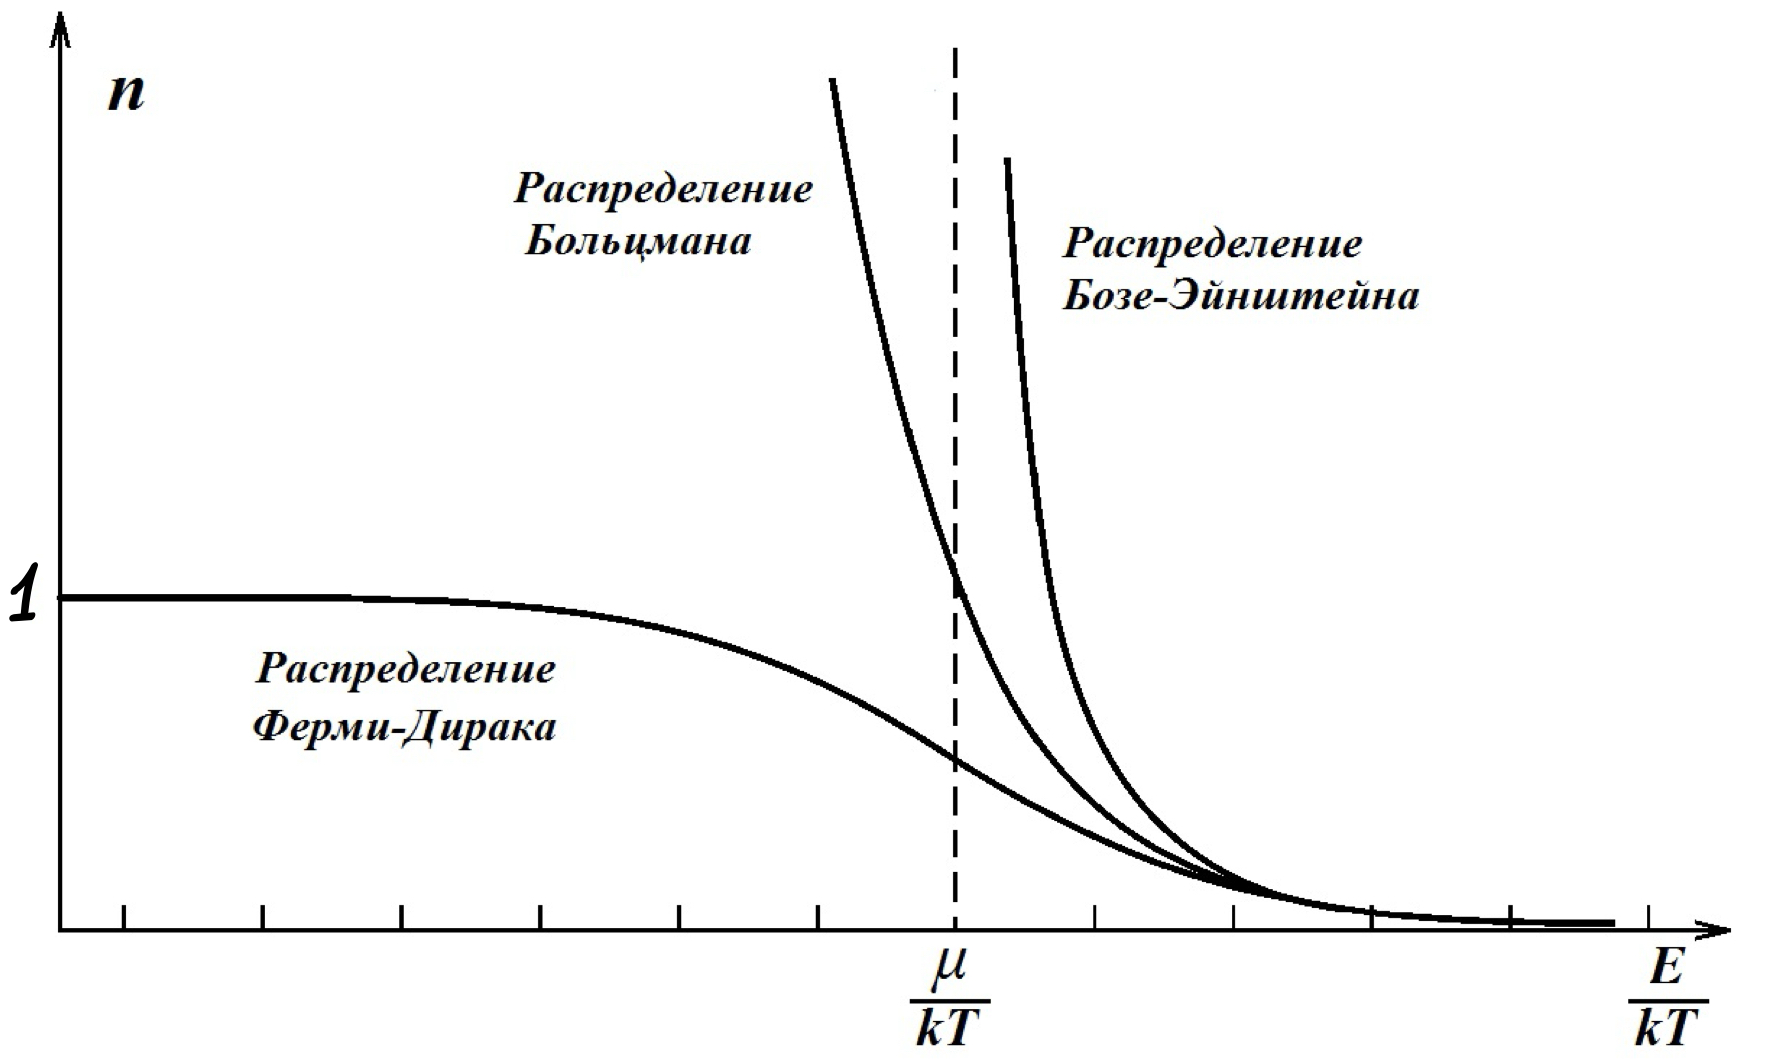
\includegraphics[width = 15cm]{stats.png}
    \end{center}

\newpage

\section{Физический смысл постоянной $\mu$}

    Рассуждения будем проводить для распределения Ферми-Дирака, так как для распределения Бозе-Эйнштейна
    всё аналогично. Вычислим химический потенциал $\mu^{*}$ ферми-газа. Для этого будем изменять число
    фермионов в системе $N$, сохраняя $T$ и $V$ постоянными. Так как предполагается, что фермионы между
    собой не взаимодействуют и объём системы постоянен, то энергетические уровни $\varepsilon_i$ и
    соответствующие им числа $Z_i$ не будут меняться. Будут меняться только числа $\overline{N_i}$.
    Приращение энтропии:
    \begin{equation*}
        dS = -k\sum\limits_{i} \ln{\frac{\overline{N_i}}{Z_i - \overline{N_i}}}d\overline{N_i} =
        -k\sum\limits_{i} \frac{\mu - \varepsilon_i}{kT} d\overline{N_i} =
        -\frac{\mu}{T}\sum\limits_{i} d\overline{N_i} + \frac{1}{T}\sum\limits_{i}\varepsilon_id\overline{N_i}
    \end{equation*}
    Следовательно:
    \begin{equation*}
        TdS = -\mu dN + dU
    \end{equation*}
    Так как $T = const$, то $d(TS) = TdS$. Поэтому:
    \begin{equation*}
        \mu dN = dU - d(TS) = d\Psi
    \end{equation*}
    Отсюда получаем:
    \begin{equation}
        \mu = \left(\frac{\partial \Psi}{\partial N}\right)_{T, V} = \mu^{*}
    \end{equation}

    Итак, доказано, что величина $\mu$ в распределениях Ферми-Дирака и Бозе-Эйнштейна является
    химическим потенциалом.

    Величину химического потенциала $\mu$ можно определить из условия нормировки:
    \begin{equation*}
        \sum\limits_{i} Z_i \overline{n_i} = \sum\limits_{i}
        \frac{Z_i}{exp\left(\frac{\varepsilon_i - \mu}{kT}\right) \pm 1} = N
    \end{equation*}
    Химический потенциал $\mu$ определён с точностью до той же произвольной аддитивной константы,
    что и энергии $\varepsilon_i$. Будем считать, что $\varepsilon_0 = 0$, тогда химический
    потенциал будет определён однозначно.

\section{Поведение ферми- и бозе-газов вблизи абсолютного нуля}

    Сначала рассмотрим ферми-газ. Из формулы \eqref{FD_distribution} видно, что для ферми-газа нет
    никаких ограничений на значение химического потенциала $\mu$. Пусть $T \longrightarrow 0$, тогда:
    \begin{equation*}
    \overline{n_i} \longrightarrow
        \begin{cases}
            1 \text{ при } \varepsilon_i < \mu    \\
            \frac{1}{2} \text{ при } \varepsilon_i = \mu  \\
            0 \text{ при } \varepsilon_i > \mu
        \end{cases}
    \end{equation*}
    Отсюда следует, что при T = 0 фермионы ферми-газа не заполняют квантовые состояния с энергиями
    $\varepsilon_i > \mu$. Про такое явление говорят, что ферми-газ находится в
    \textbf{состоянии полного вырождения}:

    \begin{center}
        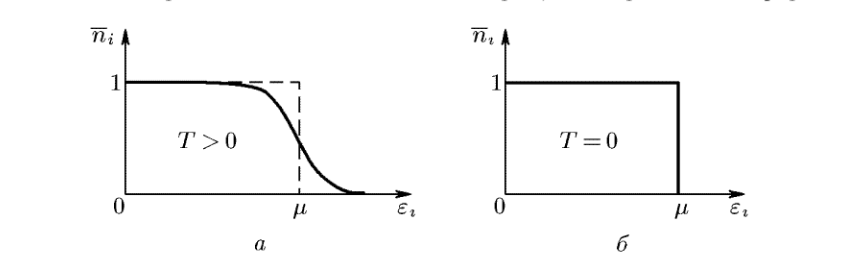
\includegraphics[width = \textwidth]{graph.png}
    \end{center}

    Теперь рассмотрим бозе-газ. Так как $\overline{n_i} \geq 0$, то, согласно формуле
    \eqref{BE_distribution}, на величину химического потенциала накладывается услвие:
    $\mu \leq \varepsilon_i$. Так как $\varepsilon_0 = 0$, то для бозе-газа $\mu \leq 0$.
    Докажем, что $\mu = 0$ при $T = 0$. Предположим, что это не так, то есть $\mu < 0$.
    Тогда при всех $i$ (в том числе при $i = 0$) разности $\varepsilon_i - \mu > 0$.
    Поэтому знаменатель в \eqref{BE_distribution} стремится к $\infty$ при $T \longrightarrow 0$,
    то есть все $\overline{n_i}\longrightarrow 0 \text{ при } T\longrightarrow 0$.
    Такое поведение наблюдается при любом числе бозонов, что невозможно. Если же $\mu = 0$ при
    $T = 0$, то в ноль обратятся только $\overline{n_i}$, где $i > 0$. Для $i = 0$ формально получаем:
    \begin{equation*}
        \overline{n_i} = \frac{1}{exp\left(\frac{0 - 0}{kT}\right) - 1} = \infty
    \end{equation*}
    На самом деле это означает, что при приближении к абсолютному нулю бозоны будут накапливаться
    на нижнем энергетическом уровне и все окажутся на нём при $T = 0$. Такое явление называется
    \textbf{бозе-эйнштейновской конденсацией}, а состояние бозе-газа - \textbf{конденсатом бозе-эйнштейна}.

\begin{center}
\begin{table}[h]
\centering
\renewcommand{\arraystretch}{1.5} % Увеличиваем высоту строк для лучшей читаемости
\begin{tabular}{|c|c|c|}
\hline
\textbf{Свойство} & \textbf{Ферми-газ} & \textbf{Бозе-газ} \\
\hline
Химический потенциал & $\mu = \varepsilon_F > 0$ & $\mu = 0$ \\
\hline
Заполнение уровней & Все уровни $\varepsilon_i < \mu$ & Все частицы в состоянии $\varepsilon_0 = 0$ \\
\hline
Квантовый эффект & Вырожденный ферми-газ & Бозе-Эйнштейн. конденсация \\
\hline
\end{tabular}
\caption{Сравнение ферми- и бозе-газов при $T = 0$}
\label{tab:fermi_bose}
\end{table}
\end{center}

\section{Вывод}

    Были получены распределения Ферми-Дирака и Бозе-Эйнштейна, а также минимально исследованы их
    свойства вблизи абсолютного нуля. Не имея информации о энергиях квантовых состояний, не
    представляется возможным исследовать эти распределения более подробно. Считаю интересным
    продолжить рассмотрение данного вопроса после знакомства с квантовой физикой в пятом семестре.
    Важно отметить, что существуют условия, при которых новая теория переходят в старую, что
    согласуется с принципом соответствия.

    Также, важно отметить, что \textbf{ферми-газы} объясняют свойства металлов, нейтронных звёзд и полупроводников.
    А \textbf{бозе-газы} описывают сверхтекучесть, сверхпроводимость и лазерные технологии, что подтверждает важность поднятой темы.

\section{Список использованной литературы}

    \begin{enumerate}
        \item Сивухин Д. В. Общий курс физики: Учеб. пособие: Для вузов. В 5 т. Т. II. Термодинамика и
        молекулярная физика. - 5-е изд., испр - М.: ФИЗМАТЛИТ, 2005. - 544 с. - ISBN 5-9221-0601-5.

        \item Петрович А.Ю. Лекции по математическому анализу. В 3-х частях: учеб. пособие. - М.:
        МФТИ, 2013. ISBN 978-5-7417-0437-0 Ч. 3. Кратные интегралы. Гармонический анализ. - 2013.
        311 с. ISBN 978-5-7417-0426-4
    \end{enumerate}

\end{document}
